\chapter{Phase speed calculations}\label{ap:SpeedCalc}

\ifpdf
    \graphicspath{{Appendices/AppendixMultiAPRcalc/PNG/}{Appendices/AppendixMultiAPRcalc/PDF/}{Appendices/AppendixMultiAPRcalc/Figs/}}
\else
    \graphicspath{{Chapter3_APR/Chapter3Figs/EPS/}{Chapter3_APR/Chapter3Figs/}}
\fi

In this appendix a calculation of the phase speed for the experimental set up in chapter~\ref{ch:MultichannelAPR}. The 2 microphones used in this example are referred to as Microphone 2 and 3, in section~\ref{sec:MultiAPRSystem}, for path $a$ and $b$ respectively. Figure~\ref{fig:SurfDiagram.pdf} shows these paths on the surface in relation to the impact site which is marked by a red dot.

\begin{figure} %SurfDiagram.pdf
\begin{minipage}[b]{1.0\linewidth}
  \centering
  \centerline{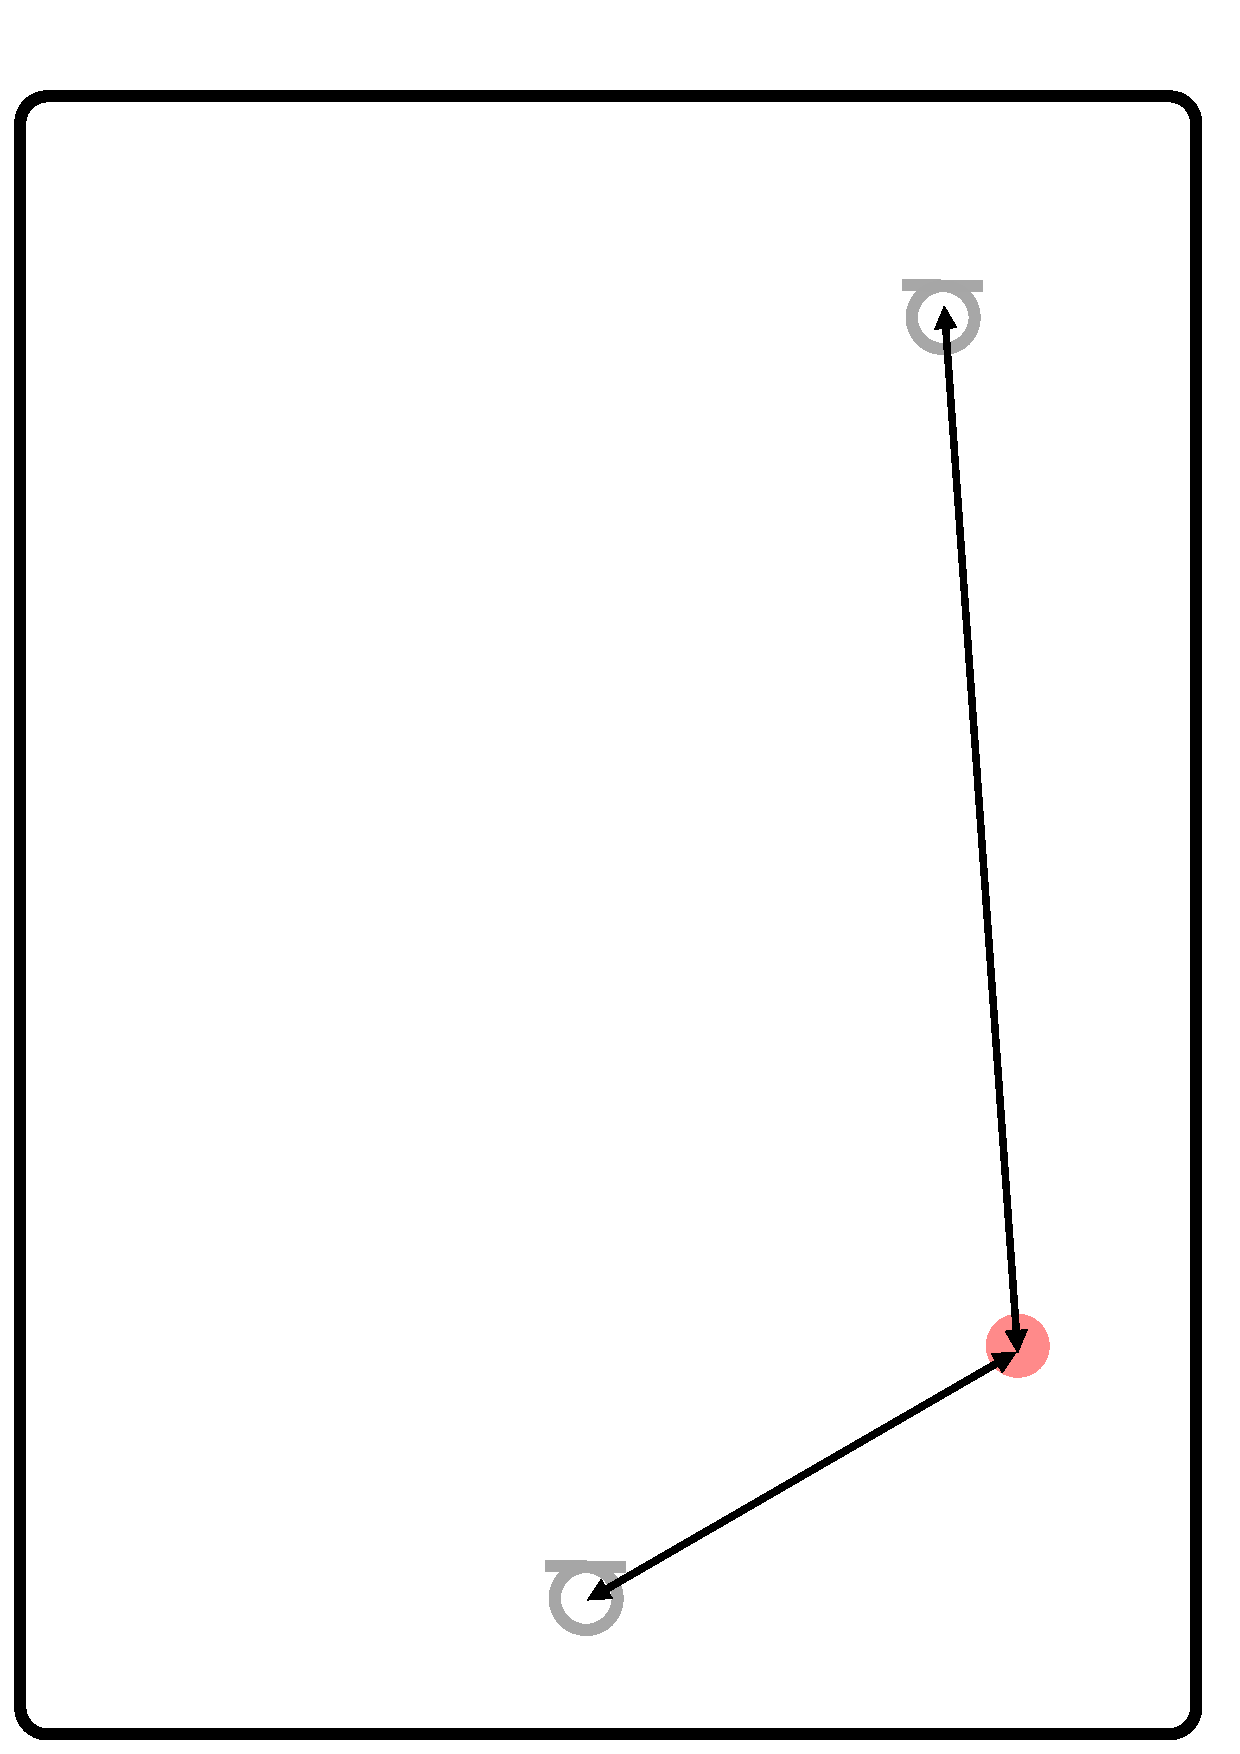
\includegraphics[width=5cm]{SurfDiagram.pdf}
  \begin{picture}(0,0)
\put(-45,100){$b$}
\put(-60,36){$a$}
\end{picture}}
\end{minipage}
\caption{Diagram of the surface with distances ($a$ and $b$) from impact site (red dot) to 2 microphones.}
\label{fig:SurfDiagram.pdf}
\end{figure}

The distances shown in Figure~\ref{fig:SurfDiagram.pdf} are as follows:
\begin{description}
  \item[$a$] 10 cm
  \item[$b$] 19.7 cm
\end{description}

While the microphones are said to be embedded in the surface the actual implementation of the microphone is a small hole drilled into the surface with the microphone wedged into it surrounded by foam. Both holes and microphones are identical and the foam surrounding them is of similar density. While the microphone diaphragms are not in direct contact with the surface the vibrations are propagated via a small gap of air to the actual microphone before being received. Given the same exact implementation of Microphone 2 and 3 the delay/time associated with this transferral is denoted $t_\theta$ for both.

We can now write the total time of flight for the impulse travelling via the two paths $t_A$ and $t_B$ as

\begin{equation}\label{eq:appPathAB}
t_A = t_a + t_\theta \qquad ; \qquad t_B = t_b + t_\theta,
\end{equation}

where $t_a$ and $t_b$ is the time of flight only within the surface material with phase speed $c$ so that

\begin{equation}\label{eq:appPathABSpeed}
t_a = \frac{a}{c} \qquad ; \qquad t_b = \frac{b}{c}.
\end{equation}

In addition the total difference in time of flight can be described as

\begin{equation}\label{eq:appPathABdif}
t_B - t_A = \Delta t = \frac{\Delta S}{f_s},
\end{equation}
for $\Delta S$ sample difference between arrival and $f_s$ sampling frequency.

The equations in \ref{eq:appPathAB} can now be substituted into equation~\ref{eq:appPathAB} and then further into~\ref{eq:appPathABdif}.

\begin{eqnarray}
% \nonumber to remove numbering (before each equation)
\nonumber   \left(\frac{b}{c} + t_\theta\right) - \left(\frac{a}{c} + t_\theta\right) &=& \frac{\Delta S}{f_s} \\
\nonumber   \frac{b-a}{c} &=& \frac{\Delta S}{f_s} \\
            c &=& \frac{f_s}{\Delta S} \left( b-a \right)
\end{eqnarray}

From Figure~\ref{fig:MultiSourceExampleAnnoSpot9.pdf} in chapter~\ref{ch:MultichannelAPR} it was found that the difference between the arrival at Microphone 2 and 3 where 11 samples, $\Delta S = 11$ at $f_s = 48000$ Hz, and given the values provided for $a$ and $b$, the phase speed $c$ in the surface was found to be $c = 423.3 $ m/s.


% ------------------------------------------------------------------------

%%% Local Variables:
%%% mode: latex
%%% TeX-master: "../thesis"
%%% End:
